\documentclass[]{article}
\usepackage{lmodern}
\usepackage{amssymb,amsmath}
\usepackage{ifxetex,ifluatex}
\usepackage{fixltx2e} % provides \textsubscript
\ifnum 0\ifxetex 1\fi\ifluatex 1\fi=0 % if pdftex
  \usepackage[T1]{fontenc}
  \usepackage[utf8]{inputenc}
\else % if luatex or xelatex
  \ifxetex
    \usepackage{mathspec}
  \else
    \usepackage{fontspec}
  \fi
  \defaultfontfeatures{Ligatures=TeX,Scale=MatchLowercase}
\fi
% use upquote if available, for straight quotes in verbatim environments
\IfFileExists{upquote.sty}{\usepackage{upquote}}{}
% use microtype if available
\IfFileExists{microtype.sty}{%
\usepackage{microtype}
\UseMicrotypeSet[protrusion]{basicmath} % disable protrusion for tt fonts
}{}
\usepackage[margin=1in]{geometry}
\usepackage{hyperref}
\hypersetup{unicode=true,
            pdftitle={R markdown},
            pdfauthor={Sébastien Renaut},
            pdfborder={0 0 0},
            breaklinks=true}
\urlstyle{same}  % don't use monospace font for urls
\usepackage{color}
\usepackage{fancyvrb}
\newcommand{\VerbBar}{|}
\newcommand{\VERB}{\Verb[commandchars=\\\{\}]}
\DefineVerbatimEnvironment{Highlighting}{Verbatim}{commandchars=\\\{\}}
% Add ',fontsize=\small' for more characters per line
\usepackage{framed}
\definecolor{shadecolor}{RGB}{248,248,248}
\newenvironment{Shaded}{\begin{snugshade}}{\end{snugshade}}
\newcommand{\AlertTok}[1]{\textcolor[rgb]{0.94,0.16,0.16}{#1}}
\newcommand{\AnnotationTok}[1]{\textcolor[rgb]{0.56,0.35,0.01}{\textbf{\textit{#1}}}}
\newcommand{\AttributeTok}[1]{\textcolor[rgb]{0.77,0.63,0.00}{#1}}
\newcommand{\BaseNTok}[1]{\textcolor[rgb]{0.00,0.00,0.81}{#1}}
\newcommand{\BuiltInTok}[1]{#1}
\newcommand{\CharTok}[1]{\textcolor[rgb]{0.31,0.60,0.02}{#1}}
\newcommand{\CommentTok}[1]{\textcolor[rgb]{0.56,0.35,0.01}{\textit{#1}}}
\newcommand{\CommentVarTok}[1]{\textcolor[rgb]{0.56,0.35,0.01}{\textbf{\textit{#1}}}}
\newcommand{\ConstantTok}[1]{\textcolor[rgb]{0.00,0.00,0.00}{#1}}
\newcommand{\ControlFlowTok}[1]{\textcolor[rgb]{0.13,0.29,0.53}{\textbf{#1}}}
\newcommand{\DataTypeTok}[1]{\textcolor[rgb]{0.13,0.29,0.53}{#1}}
\newcommand{\DecValTok}[1]{\textcolor[rgb]{0.00,0.00,0.81}{#1}}
\newcommand{\DocumentationTok}[1]{\textcolor[rgb]{0.56,0.35,0.01}{\textbf{\textit{#1}}}}
\newcommand{\ErrorTok}[1]{\textcolor[rgb]{0.64,0.00,0.00}{\textbf{#1}}}
\newcommand{\ExtensionTok}[1]{#1}
\newcommand{\FloatTok}[1]{\textcolor[rgb]{0.00,0.00,0.81}{#1}}
\newcommand{\FunctionTok}[1]{\textcolor[rgb]{0.00,0.00,0.00}{#1}}
\newcommand{\ImportTok}[1]{#1}
\newcommand{\InformationTok}[1]{\textcolor[rgb]{0.56,0.35,0.01}{\textbf{\textit{#1}}}}
\newcommand{\KeywordTok}[1]{\textcolor[rgb]{0.13,0.29,0.53}{\textbf{#1}}}
\newcommand{\NormalTok}[1]{#1}
\newcommand{\OperatorTok}[1]{\textcolor[rgb]{0.81,0.36,0.00}{\textbf{#1}}}
\newcommand{\OtherTok}[1]{\textcolor[rgb]{0.56,0.35,0.01}{#1}}
\newcommand{\PreprocessorTok}[1]{\textcolor[rgb]{0.56,0.35,0.01}{\textit{#1}}}
\newcommand{\RegionMarkerTok}[1]{#1}
\newcommand{\SpecialCharTok}[1]{\textcolor[rgb]{0.00,0.00,0.00}{#1}}
\newcommand{\SpecialStringTok}[1]{\textcolor[rgb]{0.31,0.60,0.02}{#1}}
\newcommand{\StringTok}[1]{\textcolor[rgb]{0.31,0.60,0.02}{#1}}
\newcommand{\VariableTok}[1]{\textcolor[rgb]{0.00,0.00,0.00}{#1}}
\newcommand{\VerbatimStringTok}[1]{\textcolor[rgb]{0.31,0.60,0.02}{#1}}
\newcommand{\WarningTok}[1]{\textcolor[rgb]{0.56,0.35,0.01}{\textbf{\textit{#1}}}}
\usepackage{longtable,booktabs}
\usepackage{graphicx,grffile}
\makeatletter
\def\maxwidth{\ifdim\Gin@nat@width>\linewidth\linewidth\else\Gin@nat@width\fi}
\def\maxheight{\ifdim\Gin@nat@height>\textheight\textheight\else\Gin@nat@height\fi}
\makeatother
% Scale images if necessary, so that they will not overflow the page
% margins by default, and it is still possible to overwrite the defaults
% using explicit options in \includegraphics[width, height, ...]{}
\setkeys{Gin}{width=\maxwidth,height=\maxheight,keepaspectratio}
\IfFileExists{parskip.sty}{%
\usepackage{parskip}
}{% else
\setlength{\parindent}{0pt}
\setlength{\parskip}{6pt plus 2pt minus 1pt}
}
\setlength{\emergencystretch}{3em}  % prevent overfull lines
\providecommand{\tightlist}{%
  \setlength{\itemsep}{0pt}\setlength{\parskip}{0pt}}
\setcounter{secnumdepth}{0}
% Redefines (sub)paragraphs to behave more like sections
\ifx\paragraph\undefined\else
\let\oldparagraph\paragraph
\renewcommand{\paragraph}[1]{\oldparagraph{#1}\mbox{}}
\fi
\ifx\subparagraph\undefined\else
\let\oldsubparagraph\subparagraph
\renewcommand{\subparagraph}[1]{\oldsubparagraph{#1}\mbox{}}
\fi

%%% Use protect on footnotes to avoid problems with footnotes in titles
\let\rmarkdownfootnote\footnote%
\def\footnote{\protect\rmarkdownfootnote}

%%% Change title format to be more compact
\usepackage{titling}

% Create subtitle command for use in maketitle
\newcommand{\subtitle}[1]{
  \posttitle{
    \begin{center}\large#1\end{center}
    }
}

\setlength{\droptitle}{-2em}

  \title{R markdown}
    \pretitle{\vspace{\droptitle}\centering\huge}
  \posttitle{\par}
    \author{Sébastien Renaut}
    \preauthor{\centering\large\emph}
  \postauthor{\par}
      \predate{\centering\large\emph}
  \postdate{\par}
    \date{February 26, 2019}


\begin{document}
\maketitle

\hypertarget{introduction}{%
\section{Introduction}\label{introduction}}

\begin{itemize}
\tightlist
\item
  You can download the workshop material here
  (\url{https://github.com/seb951/rmarkdown_workshop}).
\end{itemize}

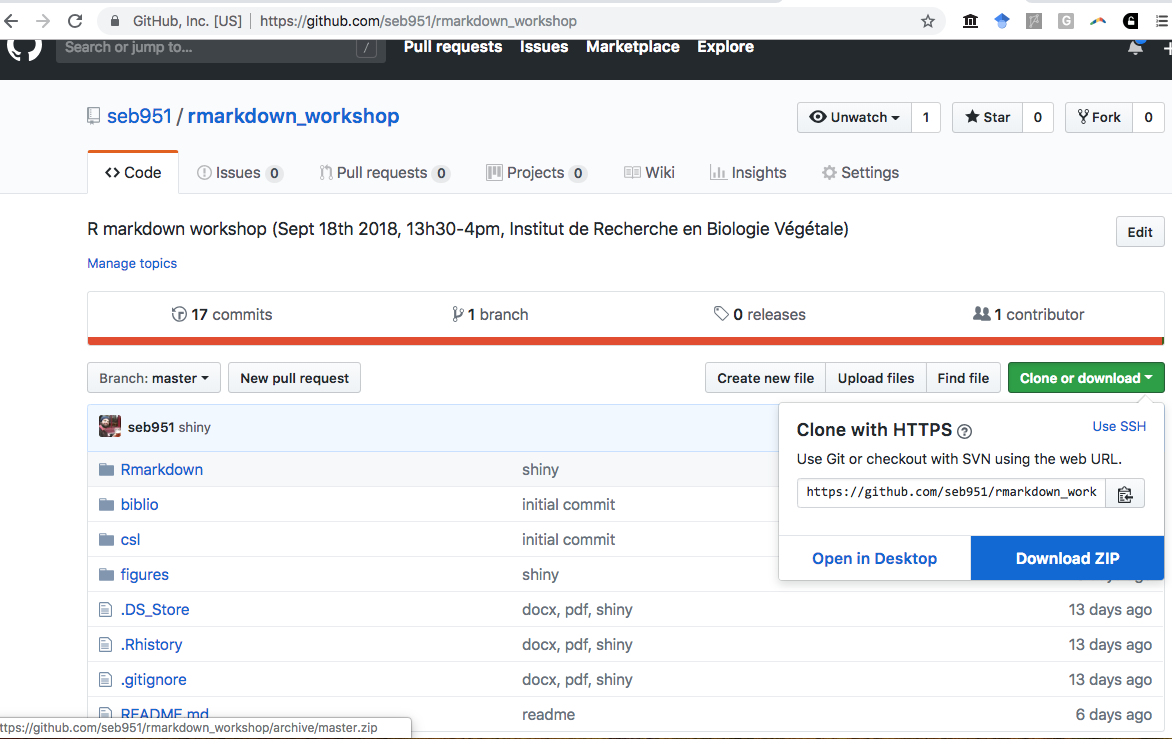
\includegraphics[width=5.20833in,height=\textheight]{../figures/download.png}\\
\hspace*{0.333em}

\begin{itemize}
\item
  Follow the \emph{.html} (web browser) and the \emph{.Rmd} (Rstudio)
  documents. Try and experiment.
\item
  \textasciitilde{}2 hours: Introduction and practice
\item
  \textasciitilde{}15 minutes: pause
\item
  \textasciitilde{}1 hour: other formats (\emph{.docx}, \emph{.pdf}).
  \href{https://seb951.github.io/rmarkdown_workshop/Rmarkdown/rmarkdown_word_pdf.html}{Workshop
  here}
\item
  \textasciitilde{}15 minutes: shiny.
  \href{https://sebastien.shinyapps.io/shiny/}{Workshop here}
\end{itemize}

\hypertarget{markdown}{%
\section{Markdown}\label{markdown}}

\begin{itemize}
\item
  Markdown is a \textbf{lightweight markup language} with plain text
  formatting syntax (Easy-to-read, easy-to-write plain text format). It
  is designed so that it can be easily converted to HTML and many other
  formats (e.g.~PDF, MS Word, .docx).
\item
  Like other markup languages (e.g.~HTML and Latex), it is completely
  independent from R.
\item
  Typically, file have the extension \emph{.md}.
\item
  Look at this
  \href{https://github.com/seb951/rmarkdown_workshop/blob/master/README.md}{example}.
  Examine the html render (github automatically interprets \emph{.md}
  files) and raw file.\\
  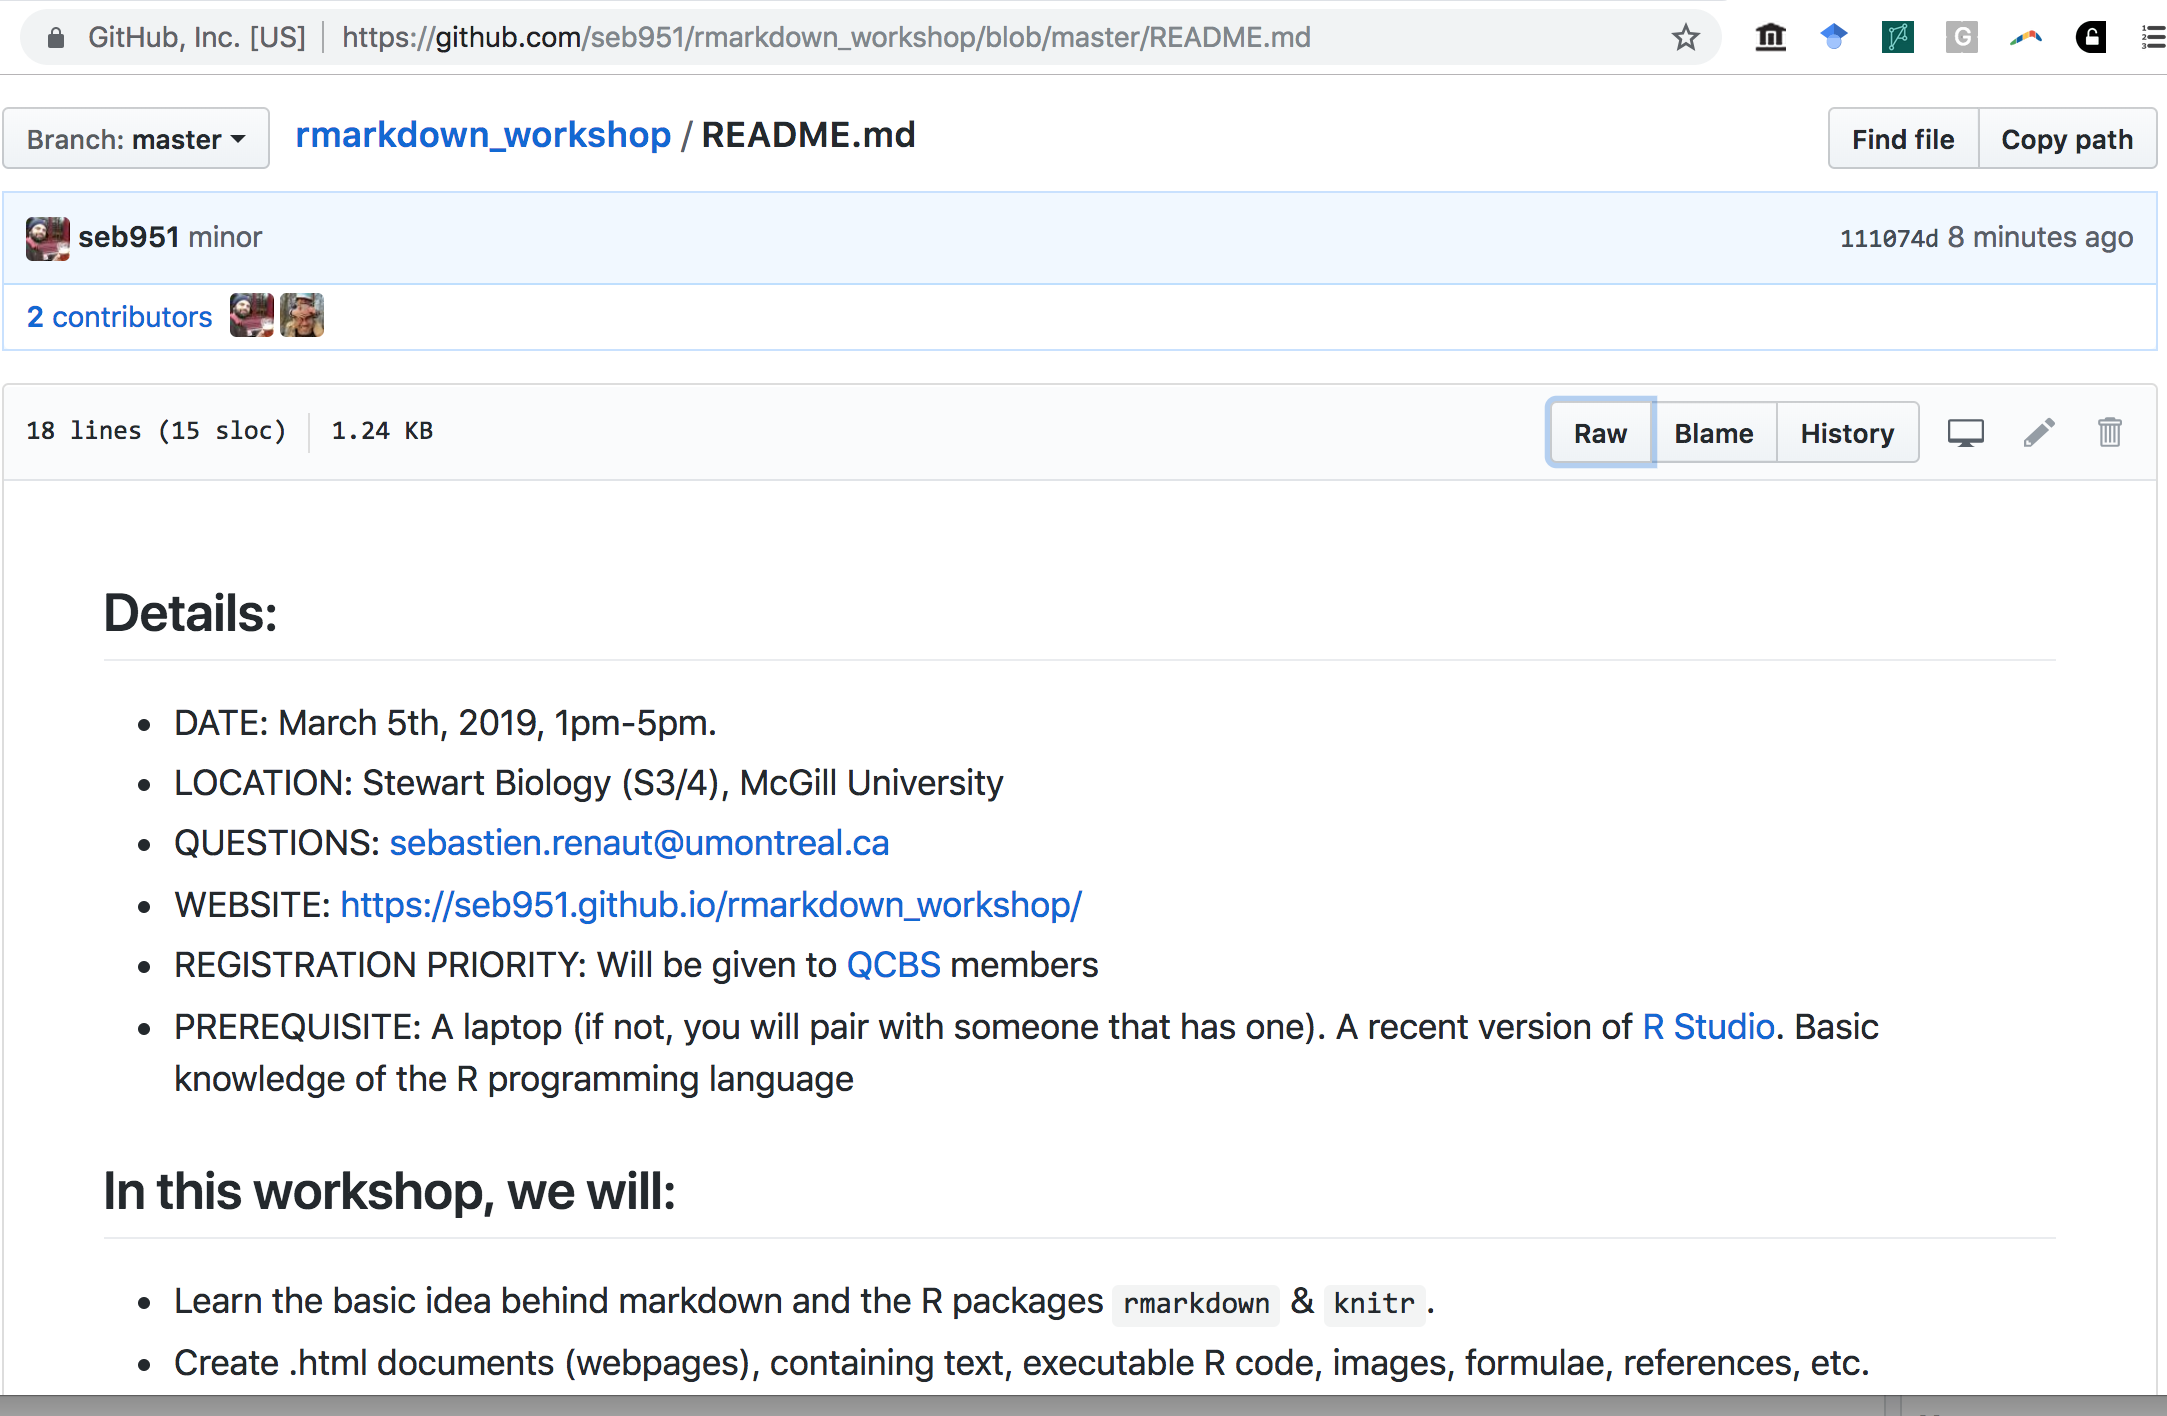
\includegraphics[width=5.20833in,height=\textheight]{../figures/md_example.png}
\end{itemize}

\hypertarget{r-markdown}{%
\section{R Markdown}\label{r-markdown}}

\begin{itemize}
\item
  An extension of the markdown syntax that enables \textbf{R code to be
  embedded and executed}.
\item
  Generate \textbf{fully reproducible reports} in different of static
  and dynamic output formats.
\item
  Most of these packages are maintained by the Rstudio team
  (\url{https://rmarkdown.rstudio.com/},
  
\includegraphics[width=0.20833in,height=\textheight]{../figures/yihui.png}
  \href{https://yihui.name/}{Yihui Xie})
\item
  Plain text files that typically have the file extension \emph{.Rmd}.
\item
  So, how does it work:

  \begin{itemize}
  \item
    Write text \& code in \texttt{Rstudio}.
  \item
    Knit: The R package \texttt{rmarkdown} feeds the \emph{.Rmd} file to
    the R package \texttt{knitr}.
  \item
    \texttt{knitr} executes code and creates a new markdown (\emph{.md})
    document which includes the code and output.
  \item
    Subsequently tranformed into \emph{.html}/\emph{.tex}/\emph{.docx}
    by \texttt{pandoc}. (Note that \emph{.tex} files need to be
    transformed by \texttt{pdflatex} into \emph{.pdf} files. We'll come
    back to that later.)
  \item
    \href{https://pandoc.org/}{\texttt{Pandoc}} is an universal document
    converter, independent of \texttt{R}.
  \item
    By default, \texttt{Rstudio} comes with \texttt{rmarkdown},
    \texttt{knitr}, and \texttt{pandoc} (but not \texttt{pdflatex}).
  \item
    When you click the \textbf{Knit} button (top left), a document will
    be generated that includes both content as well as the output of
    \texttt{R} code within the document.\\
    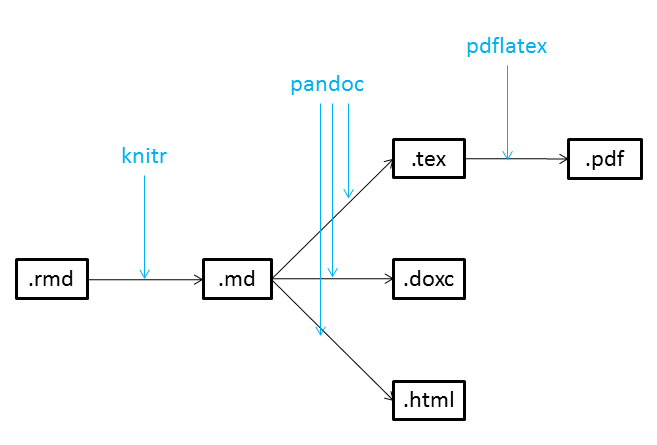
\includegraphics[width=5.20833in,height=\textheight]{../figures/pandoc1.png}
  \end{itemize}
\end{itemize}

\hypertarget{exercice-1-setting-up-an-r-markdown-file-10-min.}{%
\subsection{Exercice 1: Setting up an R markdown file (10
min.)}\label{exercice-1-setting-up-an-r-markdown-file-10-min.}}

\begin{itemize}
\tightlist
\item
  This is easily done through \texttt{R\ studio}
\end{itemize}

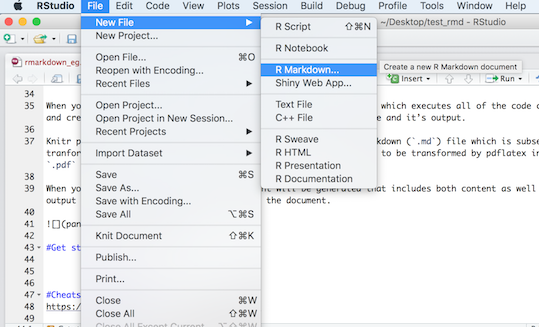
\includegraphics[width=5.20833in,height=\textheight]{../figures/getstarted.png}\\
\hspace*{0.333em}

\begin{itemize}
\item
  file \textgreater{} new file \textgreater{} R markdown \textgreater{}
  HTML
\item
  Save it (``myfirstRmarkdown.Rmd'')
\item
  Knit
\end{itemize}

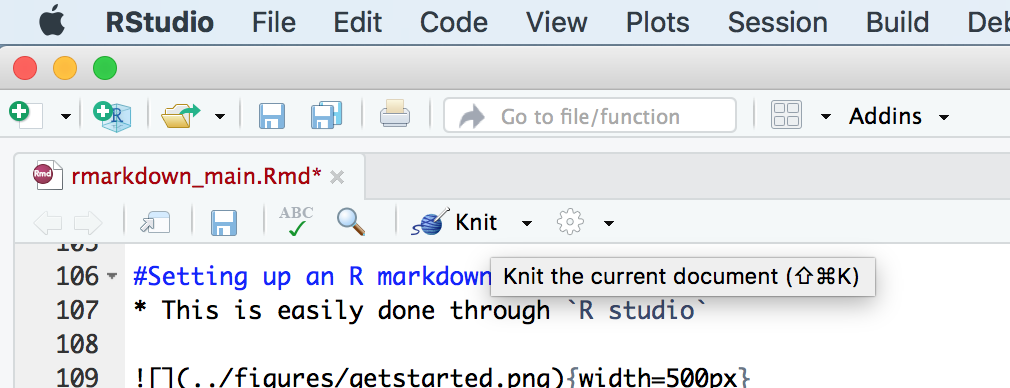
\includegraphics[width=5.20833in,height=\textheight]{../figures/knitr.png}\\
\hspace*{0.333em}

\begin{itemize}
\item
  Examine the \emph{.html} output.
\item
  Examine at the \emph{.Rmd} file structure.
\end{itemize}

\hypertarget{r-markdown-syntax}{%
\section{R markdown syntax}\label{r-markdown-syntax}}

\begin{itemize}
\item
  Markdown provides an easy way to make standard types of formatted
  text, like:

  \begin{itemize}
  \item
    \emph{italics} (*text*) or \emph{italics} (\_text\_)
  \item
    \textbf{bold} (**bold**)
  \item
    backslash (\textbackslash{}) to interpret a special characters as
    character
  \item
    \# and space at the beginning of line for a header level (6 levels,
    \# to \#\#\#\#\#\#)
  \item
    \emph{\textbf{bold italic}} (\_**bold italic**\_)
  \item
    \href{https://www.rmarkdown.rstudio.com}{links}
    ({[}links{]}(\url{https://www.rmarkdown.rstudio.com}))
  \item
    Two spaces for a newline character
  \item
    ``\&nbsp;'' character (html \emph{N}on-\emph{B}reaking \emph{SP}ace)
    for extra line spacing can be useful.
  \item
    list (first element using * and space, then \emph{idented} (tab or 2
    spaces) * and space)

    \begin{itemize}
    \tightlist
    \item
      item 1a
    \item
      item 1b
    \end{itemize}
  \item
    \texttt{quoted\ text} (`quoted text`)
  \end{itemize}
\end{itemize}

\begin{center}\rule{0.5\linewidth}{\linethickness}\end{center}

\textgreater{} Quoted text: 1st way\\
\textgreater{} more quoted text\\
\textgreater{} still more quoted text

\begin{quote}
Quoted text: 1st way\\
more quoted text\\
still more quoted text
\end{quote}

\begin{center}\rule{0.5\linewidth}{\linethickness}\end{center}

`Quoted text: 2nd way`\\
`more quoted text`\\
`still more quoted text`

\texttt{Quoted\ text:\ 2nd\ way}\\
\texttt{more\ quoted\ text}~\\
\texttt{still\ more\ quoted\ text}

\begin{center}\rule{0.5\linewidth}{\linethickness}\end{center}

```\\
\Quoted text: 3rd way\\
\more quoted text\\
\still more quoted text\\
```

\begin{verbatim}
Quoted text: 3rd way    
more quoted text         
still more quoted text        
\end{verbatim}

\begin{center}\rule{0.5\linewidth}{\linethickness}\end{center}

\begin{itemize}
\tightlist
\item
  Tables
\end{itemize}

\begin{quote}
Species \textbar{} Counts\\
--------- \textbar{} -----\\
\emph{H. sapiens} \textbar{} 24\\
\emph{M. musculus} \textbar{} 442
\end{quote}

\begin{longtable}[]{@{}ll@{}}
\toprule
Species & Counts\tabularnewline
\midrule
\endhead
\emph{H. sapiens} & 24\tabularnewline
\emph{M. musculus} & 442\tabularnewline
\bottomrule
\end{longtable}

\begin{itemize}
\tightlist
\item
  The
  \href{https://www.rstudio.com/wp-content/uploads/2015/02/rmarkdown-cheatsheet.pdf}{cheatsheet
  v1} or
  \href{\%5Bcheatsheet\%20v1\%5D(https://www.rstudio.com/wp-content/uploads/2015/02/rmarkdown-cheatsheet.pdf)}{v2}
  is your friend.
\end{itemize}

\hypertarget{exercice-2-10-min.}{%
\subsection{Exercice 2 (10 min.)}\label{exercice-2-10-min.}}

\begin{itemize}
\tightlist
\item
  Lets write some text now (add italicized/bold text, some URLs, and an
  itemized list, have fun!). Convert the document to a webpage.
\end{itemize}

\hypertarget{header}{%
\section{Header}\label{header}}

\begin{verbatim}
---  
title: "Rmarkdown"  
author: "Sebastien Renaut"  
date: '2018-03-12'  
output: html_document  
---  
\end{verbatim}

\begin{itemize}
\item
  Header, metadata, YAML, YAML Ain't Markup Language
  (\url{https://en.wikipedia.org/wiki/YAML\#History_and_name}) ?
\item
  Header specifies configurations (what kind of document will be
  created, and the options chosen).
\item
  It is not required (defaults then apply).
\item
  It uses \texttt{Python}-style indentation to specify certain options.
\item
  Many options possible depending what type of document you are
  generating. See below for some examples.
\item
  Note that some options can be specified either for the whole document
  (in the header), the code chunks, or both (chunks options supersede
  header). More on code chunks later.
\end{itemize}

\hypertarget{customizing-header}{%
\section{Customizing header}\label{customizing-header}}

\begin{verbatim}
---  
title: "Rmarkdown"  
author: "Sebastien Renaut"  
date: "February 26, 2019"   
output: 
#pdf_document:
 html_document:  
   highlight: tango  
   number_sections: T  
   theme: united 
   toc: yes  
   toc_depth: 3  
---  
\end{verbatim}

\begin{itemize}
\tightlist
\item
  Note the indentation in the \textbf{.Rmd} document for the
  \emph{output} options.
\item
  Note the \textbf{\#} symbol to comment out option.\\
\item
  Note that date is population via an \texttt{R} function
\end{itemize}

\hypertarget{outputs}{%
\subsection{Outputs}\label{outputs}}

See the
\href{https://rmarkdown.rstudio.com/lesson-9.html}{documentation} for
more information. But these are some formats of interest:

\begin{itemize}
\item
  \texttt{output:\ html\_document}
\item
  \texttt{output:\ ioslides\_presentation}
\item
  \texttt{output:\ pdf\_document} (This will require that you have a
  \href{https://www.latex-project.org/get/}{Latex software} installed -
  We'll get to that later).
\item
  \texttt{output:\ word\_document} (\emph{.docx})
\item
  interactive \texttt{shiny} apps (We'll get to that later).
\end{itemize}

\hypertarget{customizing-header-table-of-content}{%
\subsection{Customizing header: Table of
content}\label{customizing-header-table-of-content}}

\begin{itemize}
\item
  \texttt{toc:\ yes} Generate TOC.
\item
  \texttt{toc\_depth:3} depth of TOC.
\item
  \texttt{number\_sections:T} Add section numbering to headers.
\item
  More options
  \href{https://bookdown.org/yihui/rmarkdown/html-document.html\#table-of-contents}{here}
\end{itemize}

\hypertarget{customizing-header-theme-highlight-other-options}{%
\subsection{Customizing header: Theme, highlight \& other
options}\label{customizing-header-theme-highlight-other-options}}

\begin{itemize}
\item
  \texttt{theme:} specifies the theme to use for the page (``cerulean'',
  ``journal'', ``flatly'', ``readable'', ``spacelab'', ``united'', and
  ``cosmo'').
\item
  \texttt{highlight:} Syntax highlighting style (e.g. ``tango'',
  ``pygments'', ``kate'', ``zenburn'').
\item
  See this
  \href{https://www.rstudio.com/wp-content/uploads/2015/03/rmarkdown-reference.pdf}{Reference
  guide} for more options.
\end{itemize}

\hypertarget{exercice-3-10-min.}{%
\subsection{Exercice 3 (10 min.)}\label{exercice-3-10-min.}}

\begin{itemize}
\tightlist
\item
  Change theme of your \texttt{Rmarkdown} document\\
\item
  Change highlighting\\
\item
  Add TOC\\
\item
  Try saving it as \texttt{output:\ word\_document}\\
\item
  Save, knitr and play with options.
\end{itemize}

\hypertarget{code-chunks}{%
\section{Code chunks}\label{code-chunks}}

\begin{itemize}
\item
  The real power of \texttt{R\ Markdown} comes from mixing markdown with
  chunks of code.
\item
  A code chunk is intepreted by \texttt{knitr}. It works essentially the
  same as the \texttt{R} syntax we are familiar with.
\item
  A main code chunks may look like this:
\end{itemize}

\begin{quote}
```\{r code chunk example, include = T, message = T, warning=T, echo =
T, fig.cap=``Figure 1''\}\\
\#Running some R code. x = rexp(1000)\\
min(x)\\
max(x)\\
plot(x)\\
```
\end{quote}

\begin{itemize}
\item
  On the 1st line, I specify that I will run the \texttt{R} programming
  language.
\item
  Then, I give the chunk a \textbf{UNIQUE} name and specify options.
\item
  Here are common options:

  \begin{itemize}
  \item
    \texttt{include\ =\ F}: Code and results will NOT appear in the
    finished file. Code is still interpreted, and the results can be
    used by other chunks.
  \item
    \texttt{echo\ =\ FALSE} prevents code, but not results from
    appearing in the finished file. This is a useful way to embed
    figures.
  \item
    \texttt{message\ =\ FALSE} prevents messages that are generated by
    code from appearing in the finished file.
  \item
    \texttt{warning\ =\ FALSE} prevents warnings that are generated by
    code from appearing in the finished file.
  \item
    \texttt{fig.cap\ =\ "..."} adds a caption to graphical results.
  \item
    \texttt{fig.width=...}, \texttt{fig.height=...} can also change
    figure width/heigth.
  \end{itemize}
\item
  By default \texttt{R\ studio} creates a \emph{Global Options} code
  chunk. Let's examine this chunk:
\end{itemize}

\begin{quote}
```\{r setup, include=FALSE\}\\
knitr::opts\_chunk\$set(echo = TRUE)\\
```
\end{quote}

\begin{itemize}
\item
  see
  \href{https://www.rstudio.com/wp-content/uploads/2015/02/rmarkdown-cheatsheet.pdf}{cheat
  sheet} for more info.
\item
  Note that you also run inline code using the using the ` ` symbols and
  specifying the programming language. For example, ` r 10+5 ` would be
  processes as 15.
\end{itemize}

\hypertarget{exercice-4-10-min.}{%
\subsection{Exercice 4 (10 min.)}\label{exercice-4-10-min.}}

\begin{itemize}
\tightlist
\item
  Add a code chunks that will:

  \begin{itemize}
  \tightlist
  \item
    load an R package and make a plot\\
  \item
    load an R package and print some output of a function\\
  \end{itemize}
\item
  Run inline code.\\
\item
  Can you find options to print code, but not run it?\\
\item
  Also, try clicking the green arrow in the \emph{.Rmd} on the right to
  execute a code chunk a preview its output.
\end{itemize}

\hypertarget{more-code-chunks}{%
\subsection{More Code chunks}\label{more-code-chunks}}

R markdown can read and execute different languages!

\begin{itemize}
\tightlist
\item
  \textbf{bash}
\end{itemize}

\begin{Shaded}
\begin{Highlighting}[]
\FunctionTok{ls}\NormalTok{ -1}
\end{Highlighting}
\end{Shaded}

\begin{verbatim}
## rmarkdown_main.Rmd
## rmarkdown_main.html
## rmarkdown_main.log
## rmarkdown_main.tex
## rmarkdown_main_files
## rmarkdown_word_pdf.Rmd
## rmarkdown_word_pdf.html
## rmarkdown_word_pdf.pdf
## rmarkdown_word_pdf.tex
## rsconnect
## shiny.Rmd
## test.Rmd
## test.html
\end{verbatim}

\begin{itemize}
\tightlist
\item
  \textbf{python}
\end{itemize}

\begin{Shaded}
\begin{Highlighting}[]
\NormalTok{x }\OperatorTok{=} \StringTok{"hello python!"}
\BuiltInTok{print}\NormalTok{(x.split(}\StringTok{' '}\NormalTok{))}
\end{Highlighting}
\end{Shaded}

\begin{verbatim}
## ['hello', 'python!']
\end{verbatim}

\begin{itemize}
\tightlist
\item
  \textbf{perl}
\end{itemize}

\begin{Shaded}
\begin{Highlighting}[]
\FunctionTok{print} \KeywordTok{"}\StringTok{Hello perl!}\KeywordTok{"}\NormalTok{;}
\end{Highlighting}
\end{Shaded}

\begin{verbatim}
## Hello perl!
\end{verbatim}

\hypertarget{math-symbols}{%
\subsection{Math symbols}\label{math-symbols}}

Mathematical material is set off by the use of single dollar-sign
characters (similar as in the LaTeX typesetting language).

\begin{itemize}
\item
  So to write \(E = mc^{2}\), you'd write: \textbf{\$E = mc\^{}\{2\}\$}
\item
  \(\sum_{i=1}^n ASV\)
\item
  \(F_{(1,69)}\) = 1.27, \emph{p}-value=0.26
\item
  \(A = \pi*r^{2}\)
\item
  \(\sqrt{b^2 - 4ac}\)
\item
  If you wish to use a dollar sign, you need to preface it with a
  back-slash \(E = mc^{2}\) versus \$E = mc\^{}\{2\}\$
\item
  The use of double dollars quote allows for displayed formulas
  (centered). \[\sqrt{b^2 - 4ac}\]
\item
  See
  \href{http://www.math.mcgill.ca/yyang/regression/RMarkdown/example.html}{more}
  example equations from this McGill math Rmarkdown tutorial.
\end{itemize}

\hypertarget{include-pictures-figures.}{%
\section{Include pictures \& figures.}\label{include-pictures-figures.}}

\begin{itemize}
\item
  There are several ways to include figures.
\item
  Can be included from an URL directly uploaded from the web:\\
  \texttt{!{[}optional\ caption\ here{]}(https://static.independent.co.uk/s3fs-public/styles/article\_large/public/thumbnails/image/2017/09/12/11/naturo-monkey-selfie.jpg)\{width=250px\}}
\end{itemize}

\includegraphics[width=2.60417in,height=\textheight]{https://static.independent.co.uk/s3fs-public/styles/article_large/public/thumbnails/image/2017/09/12/11/naturo-monkey-selfie.jpg}\\
\hspace*{0.333em}\\
\hspace*{0.333em}\\
\hspace*{0.333em}

\begin{itemize}
\item
  If this figure is small, it can be added to the text directly: eg.:
  Today, we are using
  
\includegraphics[width=0.45833in,height=\textheight]{../figures/rstudio.png}
  to generate webpages with
  \includegraphics[width=0.3125in,height=\textheight]{https://static.independent.co.uk/s3fs-public/styles/article_large/public/thumbnails/image/2017/09/12/11/naturo-monkey-selfie.jpg}
  images\ldots{}
\item
  This is a graph previously saved in the \emph{figures} directory\\
  \texttt{!{[}{]}(../figures/DEG\_heatmap.png)\{width=250px\}}~\\
  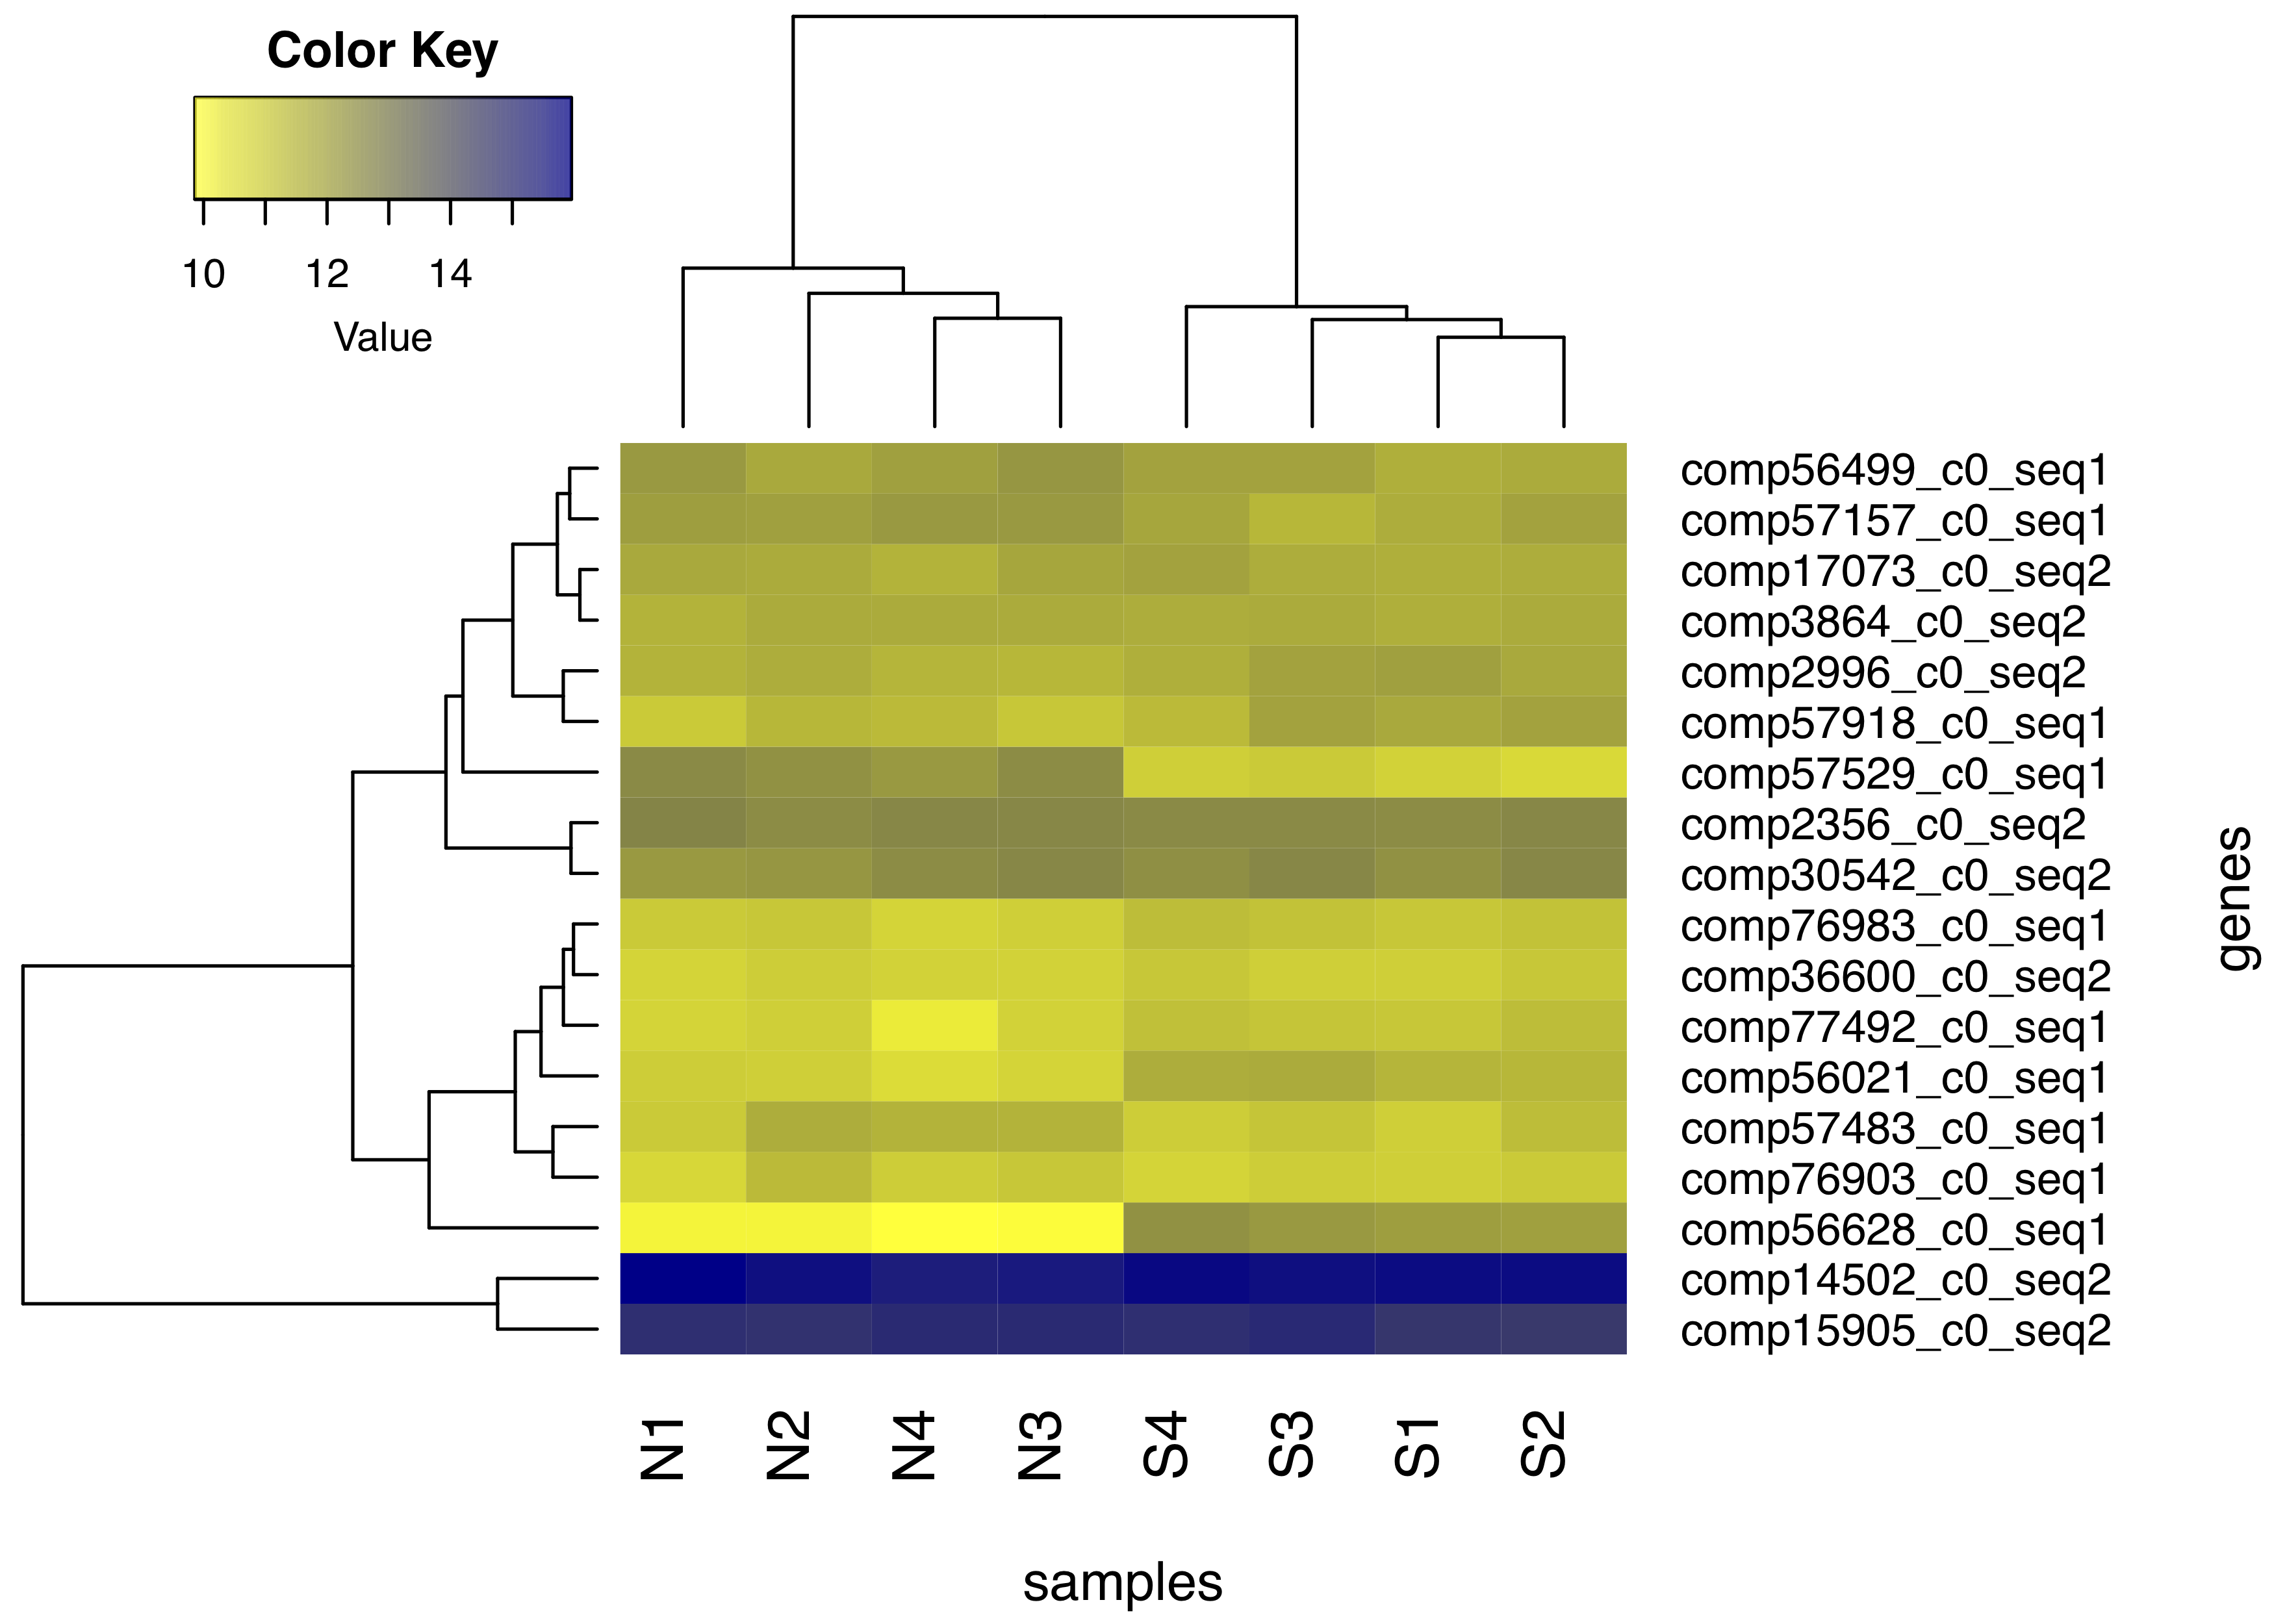
\includegraphics[width=2.60417in,height=\textheight]{../figures/DEG_heatmap.png}
  ~
\item
  In all these cases, graphs are rendered with \texttt{pandoc} and not
  \texttt{knitr}, so pandoc options need to be specified, not R graphics
  options:

  \begin{itemize}
  \item
    It's simple, but options are tricky.
  \item
    You may need to play with spacing, figure size, and figure position.
  \item
    Options are specified directly after the URL or link (eg.
    \{width=250px\} or \{width=50\%\}).
  \end{itemize}
\item
  Images can also be interpreted by \texttt{knitr} as below:
\end{itemize}

\begin{quote}
```\{r graphic\_example, out.width = ``20\%'', fig.cap = ``An orange
man'', echo = F,fig.align = ``center''\}\\
knitr::include\_graphics(``../figures/orange.jpeg'')\\
```
\end{quote}

\begin{figure}

{\centering 
\includegraphics[width=0.2\linewidth]{../figures/orange} 

}

\caption{An orange man}\label{fig:graphic_example}
\end{figure}

\begin{itemize}
\tightlist
\item
  Graphs can also be generated directly by \texttt{R} code, specified in
  a code chunk (\texttt{R} options specified in the code chunk) and
  interpreted by \texttt{knitr} as we did previously.
\end{itemize}

\begin{Shaded}
\begin{Highlighting}[]
\KeywordTok{library}\NormalTok{(ggplot2)}
\NormalTok{mtcars_ggplot =}\StringTok{ }\KeywordTok{ggplot}\NormalTok{(mtcars, }\KeywordTok{aes}\NormalTok{(}\DataTypeTok{x=}\NormalTok{wt, }\DataTypeTok{y=}\NormalTok{mpg)) }\OperatorTok{+}\StringTok{ }
\KeywordTok{geom_point}\NormalTok{() }\OperatorTok{+}\StringTok{ }\KeywordTok{geom_smooth}\NormalTok{()}
\NormalTok{mtcars_ggplot}
\end{Highlighting}
\end{Shaded}

\includegraphics{rmarkdown_main_files/figure-latex/another example-1.pdf}

\hypertarget{including-tables}{%
\section{Including Tables}\label{including-tables}}

\begin{itemize}
\item
  By default, R Markdown displays data frames and matrices as they would
  be in the R terminal (in a monospaced font).
  
\includegraphics[width=0.40625in,height=\textheight]{../figures/vomit.png}
\item
  You can use the \texttt{knitr::kable} function for additional
  formatting, as in the \emph{.Rmd} file below.
\end{itemize}

\begin{Shaded}
\begin{Highlighting}[]
\CommentTok{#Default R printout (ugly)}
\KeywordTok{print}\NormalTok{(}\KeywordTok{head}\NormalTok{(mtcars))}
\end{Highlighting}
\end{Shaded}

\begin{verbatim}
##                    mpg cyl disp  hp drat    wt  qsec vs am gear carb
## Mazda RX4         21.0   6  160 110 3.90 2.620 16.46  0  1    4    4
## Mazda RX4 Wag     21.0   6  160 110 3.90 2.875 17.02  0  1    4    4
## Datsun 710        22.8   4  108  93 3.85 2.320 18.61  1  1    4    1
## Hornet 4 Drive    21.4   6  258 110 3.08 3.215 19.44  1  0    3    1
## Hornet Sportabout 18.7   8  360 175 3.15 3.440 17.02  0  0    3    2
## Valiant           18.1   6  225 105 2.76 3.460 20.22  1  0    3    1
\end{verbatim}

\begin{Shaded}
\begin{Highlighting}[]
\CommentTok{#With kable function from knitr (better looking)}
\NormalTok{knitr}\OperatorTok{::}\KeywordTok{kable}\NormalTok{(}\KeywordTok{head}\NormalTok{(mtcars),}\DataTypeTok{digits =}\DecValTok{1}\NormalTok{,}\DataTypeTok{caption =} \StringTok{"A motorcars table"}\NormalTok{)}
\end{Highlighting}
\end{Shaded}

\begin{longtable}[]{@{}lrrrrrrrrrrr@{}}
\caption{A motorcars table}\tabularnewline
\toprule
& mpg & cyl & disp & hp & drat & wt & qsec & vs & am & gear &
carb\tabularnewline
\midrule
\endfirsthead
\toprule
& mpg & cyl & disp & hp & drat & wt & qsec & vs & am & gear &
carb\tabularnewline
\midrule
\endhead
Mazda RX4 & 21.0 & 6 & 160 & 110 & 3.9 & 2.6 & 16.5 & 0 & 1 & 4 &
4\tabularnewline
Mazda RX4 Wag & 21.0 & 6 & 160 & 110 & 3.9 & 2.9 & 17.0 & 0 & 1 & 4 &
4\tabularnewline
Datsun 710 & 22.8 & 4 & 108 & 93 & 3.8 & 2.3 & 18.6 & 1 & 1 & 4 &
1\tabularnewline
Hornet 4 Drive & 21.4 & 6 & 258 & 110 & 3.1 & 3.2 & 19.4 & 1 & 0 & 3 &
1\tabularnewline
Hornet Sportabout & 18.7 & 8 & 360 & 175 & 3.1 & 3.4 & 17.0 & 0 & 0 & 3
& 2\tabularnewline
Valiant & 18.1 & 6 & 225 & 105 & 2.8 & 3.5 & 20.2 & 1 & 0 & 3 &
1\tabularnewline
\bottomrule
\end{longtable}

\hypertarget{exercice-5-10-min.}{%
\subsection{Exercice 5 (10 min.)}\label{exercice-5-10-min.}}

\begin{itemize}
\item
  Find a picture on the web.
\item
  Add it to document using either \texttt{knitr} or \texttt{pandoc}.
\item
  Add a table using \texttt{knitr}.
\end{itemize}

\hypertarget{citations-footnotes-bibliography}{%
\section{Citations, footnotes,
bibliography}\label{citations-footnotes-bibliography}}

\begin{itemize}
\item
  Footnotes are easy when you have a few references. Use
  \texttt{{[}\^{}1{]}} and add reference at the end using same
  format.\footnote{Renaut 2019. R markdown footnoe. Number 1. pp1-2}
\item
  Otherwise, you may specify a bibliography and citation style in the
  header.
\end{itemize}

\texttt{-\/-\/-}\\
\texttt{csl:\ csl/peerj.csl}~\\
\texttt{bibliography:\ biblio/test\_library.bib}~\\
\texttt{-\/-\/-}

\begin{itemize}
\item
  The Citation Style Language (\emph{.csl}) file specifies the reference
  format.
\item
  It is an open XML-based language to describe the formatting of
  citations and bibliographies. Reference management programs using
  \emph{.csl} include Zotero, Mendeley and Papers.
\item
  Most journals should have a \emph{.csl} file be on this
  \href{https://github.com/citation-style-language/styles}{github repo}.
  But you could create your own.
\item
  A \emph{.bib} file contains the bibliographic information of your
  document.
\item
  Here, I created a a \emph{.bib} file in the reference management
  software \href{https://www.readcube.com/papers/mac}{Papers3}.
\item
  But now, I often copy \emph{.bib} reference directly from google
  scholar.\\
  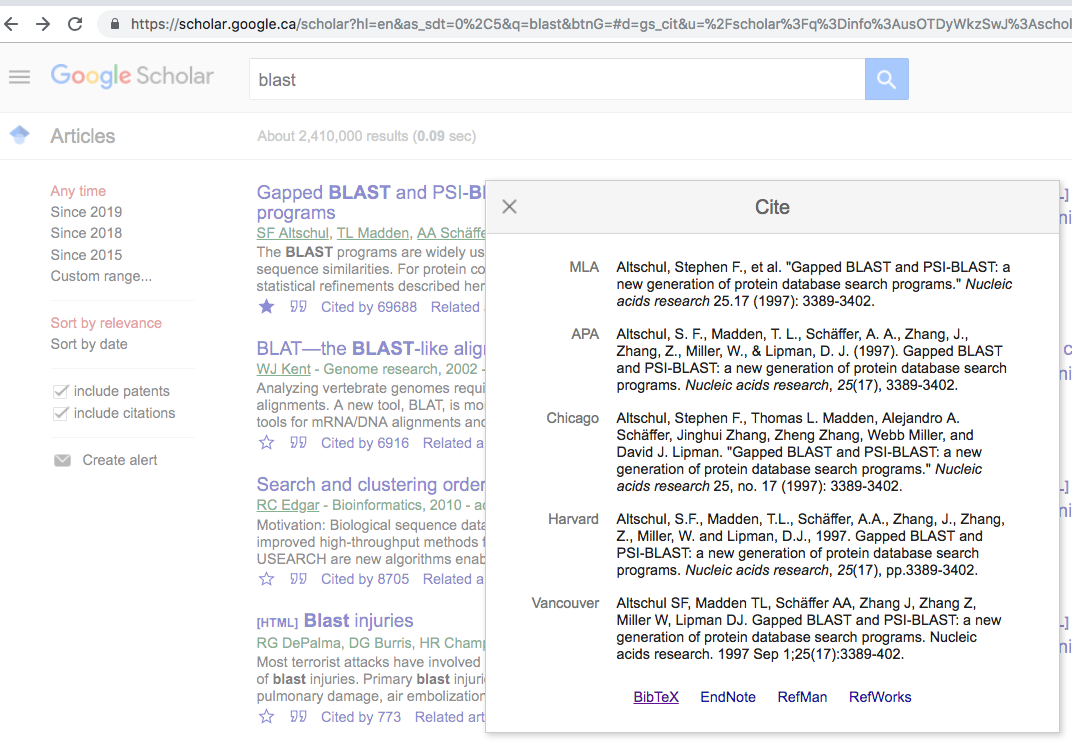
\includegraphics[width=5.20833in,height=\textheight]{../figures/gs.png}
\end{itemize}

\hypertarget{citations-examples}{%
\subsection{Citations: examples}\label{citations-examples}}

\begin{itemize}
\item
  Example: The bioinformatics program \emph{BLAST} (Altschul et al.,
  1997) has been cited nearly 70,000 times!
\item
  These are three random references (eg. Thibert-Plante \& Hendry, 2010;
  Wagner et al., 2012; Yoshida et al., 2014).
\item
  Citations go inside square brackets {[} {]} and are separated by
  semicolons (;).
\item
  Each citation must have a unique key, composed of `@' + the citation
  identifier from the \emph{.bib} database.
\item
  A minus sign (-) before the @ will suppress mention of the author in
  the citation. This can be useful when the author is already mentioned
  in the text. For example, Stephen Altschul and a bunch of other people
  (1997) have been cited 70,000 times.
\end{itemize}

\hypertarget{exercice-6-10-min.}{%
\subsection{Exercice 6 (10 min.)}\label{exercice-6-10-min.}}

\begin{itemize}
\item
  Create a library (\texttt{.bib} file) with the references for your
  five favorite scientific papers.
\item
  Find and use another Citation Style Language (e.g.~Nature, PLOS ONE,
  Indian Journal Of Dermatology, etc.).
\end{itemize}

\hypertarget{cheatsheets-and-help}{%
\section{Cheatsheets and help}\label{cheatsheets-and-help}}

\begin{itemize}
\item
  \href{https://rmarkdown.rstudio.com/lesson-1.html}{Lessons}
\item
  \href{https://bookdown.org/yihui/rmarkdown/}{Book}
\item
  \href{https://www.rstudio.com/wp-content/uploads/2015/02/rmarkdown-cheatsheet.pdf}{Cheatsheet
  (old - short)}
\item
  \href{https://www.rstudio.com/wp-content/uploads/2016/03/rmarkdown-cheatsheet-2.0.pdf}{Cheatsheet
  (newer - longer)}
\item
  \href{https://holtzy.github.io/Pimp-my-rmd/}{Pimp my Rmd}
\item
  \href{https://stackoverflow.com/}{Stack Overflow}
\end{itemize}

\hypertarget{references}{%
\section{References}\label{references}}

(Note that references below are generated automatically, except for the
footnote.)

\hypertarget{refs}{}
\leavevmode\hypertarget{ref-altschul1997gapped}{}%
Altschul SF., Madden TL., Schäffer AA., Zhang J., Zhang Z., Miller W.,
Lipman DJ. 1997. Gapped blast and psi-blast: A new generation of protein
database search programs. \emph{Nucleic acids research} 25:3389--3402.

\leavevmode\hypertarget{ref-ThibertPlante:2010vw}{}%
Thibert-Plante X., Hendry A. 2010. The consequences of phenotypic
plasticity for ecological speciation. \emph{Journal Of Evolutionary
Biology}:1--17.

\leavevmode\hypertarget{ref-Wagner:2012hw}{}%
Wagner CE., Keller I., Wittwer S., Selz OM., Mwaiko S., Greuter L.,
Sivasundar A., Seehausen O. 2012. Genome-wide RAD sequence data provide
unprecedented resolution of species boundaries and relationships in the
Lake Victoria cichlid adaptive radiation. 22:787--798.

\leavevmode\hypertarget{ref-Yoshida:2014bn}{}%
Yoshida K., Makino T., Yamaguchi K., Shigenobu S., Hasebe M., Kawata M.,
Kume M., Mori S., Peichel CL., Toyoda A., Fujiyama A., Kitano J. 2014.
Sex Chromosome Turnover Contributes to Genomic Divergence between
Incipient Stickleback Species. \emph{PLoS Genetics} 10:e1004223.


\end{document}
